\documentclass[12pt]{article}
\usepackage{ugssyllabus}

\begin{document}
\pagenumbering{gobble}
\smjsyllabus{
  title  = {The \UgS Syllabus},
  author = {Omar Elshinawy},
  date   = {Spring 2025},
}

\begin{smjsyllabusabstract}
Is the game of Chess solvable? Should we be worried about the recent advances in cryptography? And, how does maths predict stock prices? With many questions in mind, the Mathematics Undergraduate Seminar (UgS) brings in student speakers to talk about interesting mathematics that not standardly found within the classroom. This syllabus structures the undergraduate seminar procedure in a seamless manner, and outlines its core processes.
\end{smjsyllabusabstract}
% ToC and \newpage emitted automatically by \end{smjsyllabusabstract}.
\pagenumbering{arabic}
%

\section{Structure.} The \UgS procedure consists of three P's,

\subsection{1. Pick a topic.} For this, you would first like to identify a main area of interest. This is done in a one-on-one meeting, where you inform me of some of your interests beforehand. Then, we may try to find a suitable learning project.

\subsection{2. Prepare an article.}
Once a topic is assigned, you will be given a clear goal. This might be to prove a statement, study a phenomenon, solve a certain probelm, or comment on a specific piece of work.

\begin{example}
     Prove theorem 2.22 in [1]. \hfill \emph{[1] = some piece of literature}
\end{example}

\noindent
Each project is accompanied by a set of resources, with guidelines. Note, however, that the goal may be reached in whatever way you'd like. Feel free to use your own material, consult the large language model, or \dots

\noindent
Your article is a formalised set of notes. There, you may dive into all the necessary constructions, cite all the theorems you need, define all the objects you like, and so on. This is your canvas of ideas, where you have all the time in the world to discuss all the things you'd like to discuss\footnote{Note that in contrast, a talk is 25$-$30 minutes, therefore you will very likely only get to share a glimpse of all the complicated constructions and rich ideas in your article.}. In a sense, this article gives you the space to list down all components, and is an opportunity to decide which components are most crucial to your project.

\noindent
A draft report is due before the talk, see \textbf{(\ref{deliverable-2})} for a comprehensive guide.

\subsection{3. Present a talk.} The first step towards this is preparing a good abstract, see \textbf{(\ref{deliverable-1})}. This shows that you know what you're talking about, clearly a necessary condition for the success of your talk.

\noindent
Next, you should schedule a meeting to \textbf{mock a presentation}. From there you get a consistent loop of feedback, one that would greatly improve the quality of your presentation. This has to be done \textbf{at least once before the talk}, but you could in principle mock more than one presentation if the time permits.

\newpage

\section{Deliverables.} As outlined in this agenda's abstract, you need to prepare the following.

\subsection{1. Abstract,}\label{deliverable-1} \hfill \emph{a few words on the contents of your talk.}\\

\noindent
Here is an example from a talk on \href{https://en.wikipedia.org/wiki/Zermelo%27s\_theorem\_(game_theory)}{Zermelo's Theorem in Game Theory}\footnote{I linked an article to give more context.},
    \begin{example}
        \begin{center}
        \begin{itemize}
            \item[] We already know that tic-tac-toe is a solved game, meaning it is determined if both players play their best. This is, however, not so clear for the game of Chess. We will first start with a good game of tic-tac-toe, then refine the intuition into rigor on our way to proving the first formal theorem in the theory of games, credited to Ernst Zermelo. In full generality, we show that in two-player finite games of perfect information, there is always a strategy to reach a win or draw; with no regard to what the strategy should be. One could then ask the following question. Given a winning position, how quickly can a win be forced? We conclude the talk with a reflection on Zermelo's findings as well as the powerful, non-intuitive consequences of his results.\footnote{Zermelo's Theorem in Game Theory, \href{https://elshenawyom.github.io/assets/pdf/zermelo\_paper.pdf}{article by myself.} A prehistoric \UgS contribution!}
        \end{itemize}
        \end{center}
        Perhaps that was a bit more than a few words. Buckle up, because this talk is converging to a boring poetry class. You see, it is very rare that you find an abstract starting with \emph{tic-tac-toe}. People have a very short attention span, and it is important to get the audience hooked. You should give immense importance to your abstract, since only a good one will attract people to show up to your talk (and read your paper afterwards). For some people\footnote{I=some people.}, it is as important as your full talk.\\[6pt]
        In another sense, notice that this abstract gives a sense of what to expect from the talk. Precisely, we have
        \begin{multicols}{2}
        \begin{enumerate}
            \item A game of \emph{tic-tac-toe},
            \item Formalisation (Definitions, \dots)
            \item Proof of Zermelo's Theorem
            \item \textbf{Bonus!} Question \& Reflection
        \end{enumerate}

        \end{multicols}
        \noindent
        and I would like to stop at the bonus part. While I did prepare more material, the reflection part is left there for flexibility. If my talk was too short, I would include the bonus part. Otherwise, I would conclude at Zermelo's Theorem. In the end, it did take me some time, and I could not discuss the bonus part. This is completely fine, since I was able to include it in my paper report, \href{https://elshenawyom.github.io/assets/pdf/zermelo\_paper.pdf}{in section 3}.
    \end{example}

\newpage

To conclude, the abstract checks the following boxes.

\emph{The abstract...}
\begin{itemize}
    \item[[~]] hooks the reader. \hfill \emph{The first sentence is your hook. Ask an interesting question, or motivate a difficult problem.}
    \item[[~]] motivates the talk. \hfill \emph{Why is it interesting? }
    \item[[~]] overviews its contents. \hfill \emph{What should I expect?}
    \item[[~]] poses (or answers) a question to invoke curiosity\footnote{While writing this, I had this \href{https://mathoverflow.net/a/210344}{exact} example in mind. Your math might be boring, but if it answers an interesting question (Factorizing integers, Predicting Stock Prices, ...) then you can make this the highlight of your abstract (and thus your talk).}. \hfill \emph{Bonus.}
\end{itemize}
Finally, I would like to note that by no means do I pose myself as an expert on the topic, nor would I like to exemplify myself. This is merely a guide, and I would be greatly interested to see what new ideas you might bring to your abstract. Let me link a few more resources.\\

\textbf{More Resources.}

\begin{enumerate}
\item \href{https://mathoverflow.net/questions/210340/how-to-write-an-abstract-for-a-math-paper}{Writing a good abstract.}\hfill \emph{Quite an interesting discussion.}
\item \href{https://elshenawyom.github.io/seminars-talks/}{My website.} \hfill \emph{Has a couple of more abstracts.}
\end{enumerate}

\newpage

\subsection{2. Report Draft,}\label{deliverable-2} \hfill \emph{Marking your progress so far.}\\

\noindent
This is more or less a crash course on writing a paper. For the draft, I only expect you to "sort" your notes according to some structured set of sections. The writing does not need to be rigorous, or well-written, or even in full sentences. All that is needed is to review your note-taking and research process, and perhaps assess your understanding of the probelm on a basic level. The goal is not to judge you, but to give you feedback on things you do well, and other things you might need to work on.

\subsubsection{Structure}
The very-first step is to structure your document. This is best demonstrated by an example.
\begin{center}
    \begin{itemize}
        \item[] \textbf{0. Preliminaries}\\
        \emph{Use this to define the baseline knowledge for your paper. For example, if you are writing a paper on linear algebra, you assume that everyone knows what a basis is.}
        \item[] \textbf{1. Motivation}\\
        \emph{What makes the problem interesting? Here, you should try to answer that question. If you have seen an interesting pattern of examples, you can use those to motivate the study. Or, if your mathematics e.g. predicts something interesting, then you should use the consequences to motivate your pursuit of the topic.}
        \item[] \textbf{2. Literature/Problem Statement}\\
        \emph{Mathematics is the work of many, many people. No matter how far down the chain you go, there is always something to cite without proof. If applicable, use this section to mention results that are relevant for your paper, which you personally don't want to spend time on (in order to e.g. save time).}
        \begin{example}
            It is known that x and y proved that all objects of this type are abc. Further, z and l used this previous result to make a general statement about this object. In this paper, we borrow these two facts, and pose the following question: (\dots)
        \end{example}
        \item[] \textbf{3. Main Theorem/Main Result}\\
        \emph{State your theorem (without proof!) The proof is usually delayed to another section of the paper}
        \item[] \textbf{4. Proof of Theorem }\\ \emph{more mathematics, the name of this section can greatly vary. As an example, it could be the phenomena you are studying.}
        \item[] \textbf{5. Future Work}\\ \emph{Generalising a result, or exploring another direction, if applicable}
        \item[] \textbf{Bibliography} \hfill \emph{always credit the authors!}
        \item[] \textbf{Acknowledgements} \hfill \emph{if any}
    \end{itemize}
\end{center}
Let me note once again that this is merely a guide. Sometimes, section 1 and 2 merge, and other times section 4 is not necessary. With proper reason, you are more than encouraged to deviate from this. Next me attach some examples from my rather humble experience.
\begin{example}[Tables of Contents] A first example is the following,
\begin{center}
    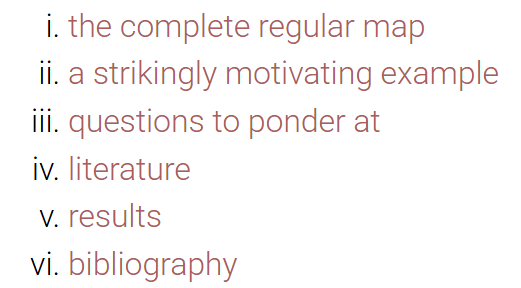
\includegraphics[width=0.45\textwidth]{assets/exmp-1-toc.png}
\end{center}
In \emph{(i)}, we define the object of interest. The following section (rather the following two sections) motivate the study of this object. Then, formalisation begins by "borrowing" from other authors' literature as in \emph{(iv)}. Finally, the results are stated in \emph{(v)}, without proof (funny enough). \hfill \href{https://elshenawyom.github.io/news/jmm2025/#research}{\emph{more here.}}
\begin{center}
    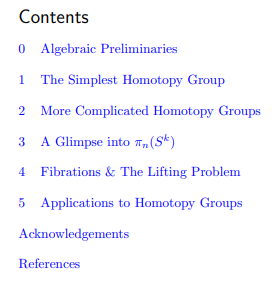
\includegraphics[width=0.45\textwidth]{assets/exmp-2-toc.png}
\end{center}
We start by defining a baseline for the discussion in section zero. Next, sections 1 to 3 introduce the problem on different levels. Section 4 formalises the problem and proves the relevant results, then these results are applied in the final section. \hfill \href{https://elshenawyom.github.io/assets/pdf/fibrations\_paper.pdf}{\emph{more here.}}
\begin{center}
    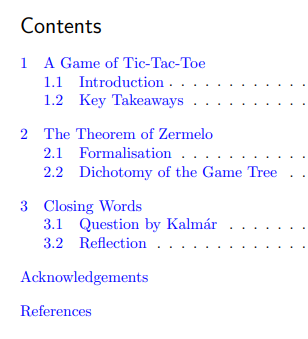
\includegraphics[width=0.45\textwidth]{assets/exmp-3-toc.png}
\end{center}
This is the \emph{tic-tac-toe} example. The motivation section is disguised under this Tic-Tac-Toe game. Then, the statement and proof of the theorem is mentioned. Finally, a reflection and consequences section is there to give some more ideas. \href{https://elshenawyom.github.io/assets/pdf/zermelo\_paper.pdf}{\emph{more here.}}
\begin{center}
    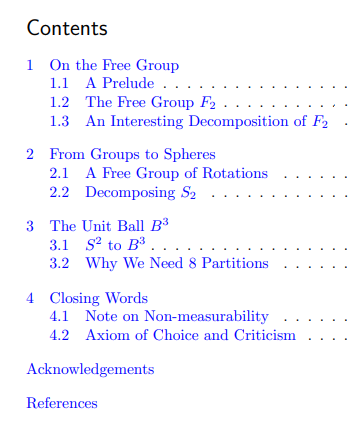
\includegraphics[width=0.45\textwidth]{assets/exmp-4-toc.png}
\end{center}
The first section motivates the discussion by introducing \emph{an interesting decomposition}. Then, this idea is applied to the construction in sections 2 and 3. Finally, the closing words section reflects on some ideas used in the proof, and gives historical context by means of a story.  \hfill  \href{https://elshenawyom.github.io/assets/pdf/banachtarski\_paper.pdf}{\emph{more here.}}
\end{example}
\noindent
With these examples in mind, I hope this was a clear communication of ideas.
\subsubsection{Take Notes}

This seems obvious, but you should start writing down notes on many of the things you find to be interesting. Funny enough, this is what they call research\footnote{in a sense}. You need to write \textbf{a lot} of things, either by rewriting a statement in your own words, or filling in logical gaps in a proof you read. You should treat your draft as your mathematical diary, yet to be polished and structured later on. A good starting point is to review the existing literature.

\subsubsection{Re-iterate}
Most of the work lies in proper structuring/sectioning. Writing is a creative process, and so your document structure will naturally change with time, depending on your notes and findings.

\section{Closing Words.} This syllabus transforms insight and experience into useful examples and well-articulated guidelines. Nevertheless, if you still have questions, this is completely okay. Please reach out with questions! \hfill $\boxed \xi$

\end{document}